
\subsubsection[Density-based (Mean shift)]{Density-based \textit{(Mean shift)}}
\begin{frame}

	\frametitle{{\color{GradientDescentDiagramRed}Density-based Clustering}, in sintesi}

	%\begin{block}{}
		Il density-based clustering collega aree ad alta densità in cluster. Ciò consente distribuzioni di forma arbitraria purché sia possibile collegare aree dense.
		\newlinedouble
		Questi algoritmi hanno difficoltà con dati a densità variabile e dimensionalità elevate. Inoltre, per costruzione, questi algoritmi non riescono ad assegnare dei valori anomali ai cluster.
		\begin{figure}[!htbp]
			\centering
			\includegraphics[width=5.0cm]{images/unsupervised/types/Clustering_Density.pdf}
					%\caption{Stripe Radar for Fraud Detection}
		\end{figure}
	%\end{block}

\end{frame}


\begin{frame}

	\frametitle{{\color{GradientDescentDiagramRed}Density-based Clustering}}

	%\begin{block}{}
		\begin{itemize}
			\item gli spazi delle features strutturati arbitrariamente dovrebbero essere analizzati solo attraverso metodi non parametrici che non hanno presupposti incorporati (l'adattamento della distribuzione in figura con un GMM fallirebbe)
		\end{itemize}

		\begin{columns}

			\column{0.5\linewidth}
			\begin{figure}[!htbp]
				\centering
				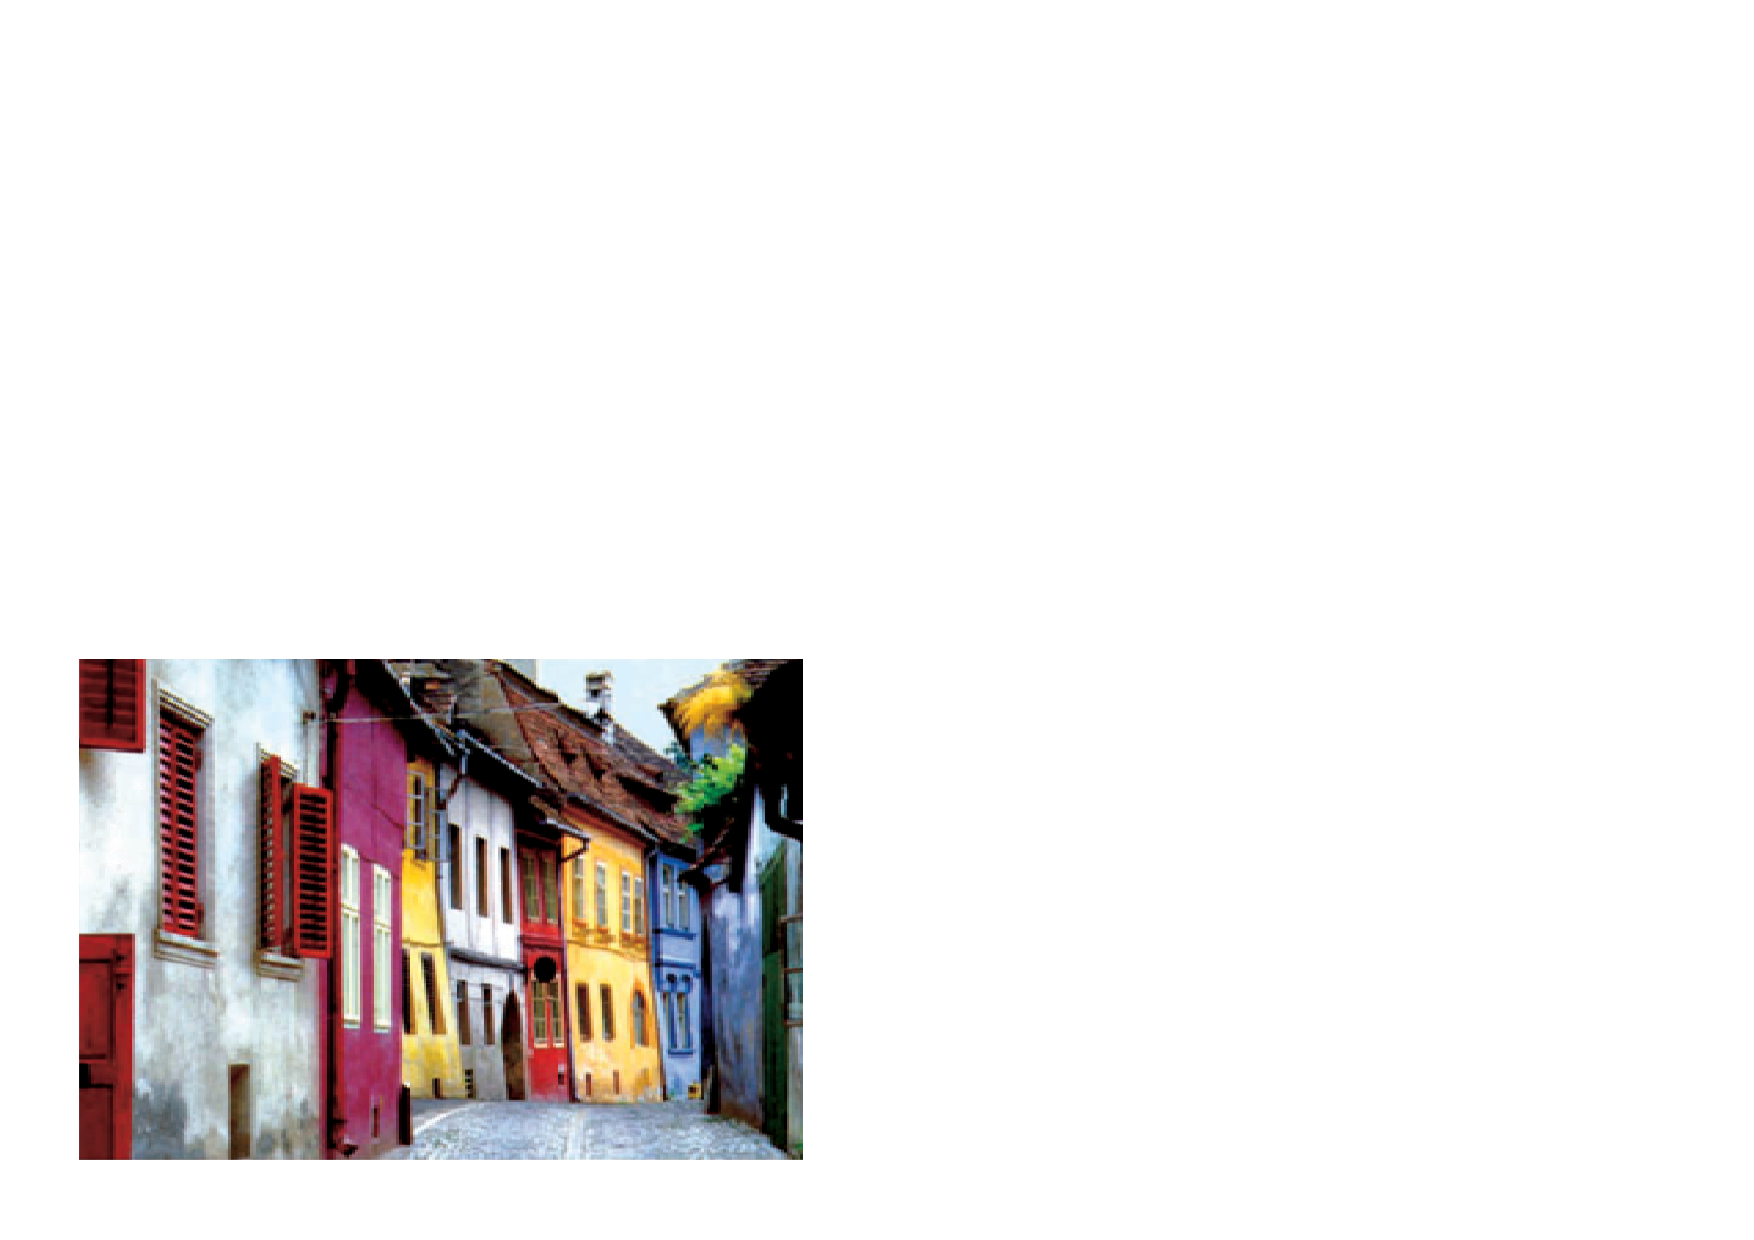
\includegraphics[width=1.0\linewidth]{images/unsupervised/non_parametric/np_1.pdf}
				%\caption{ENEL QQ-Plot Normale}
				%\label{Enel_QQ_Plot_Normal}
			\end{figure}

			\column{0.5\linewidth}
			\begin{figure}[!htbp]
				\centering
				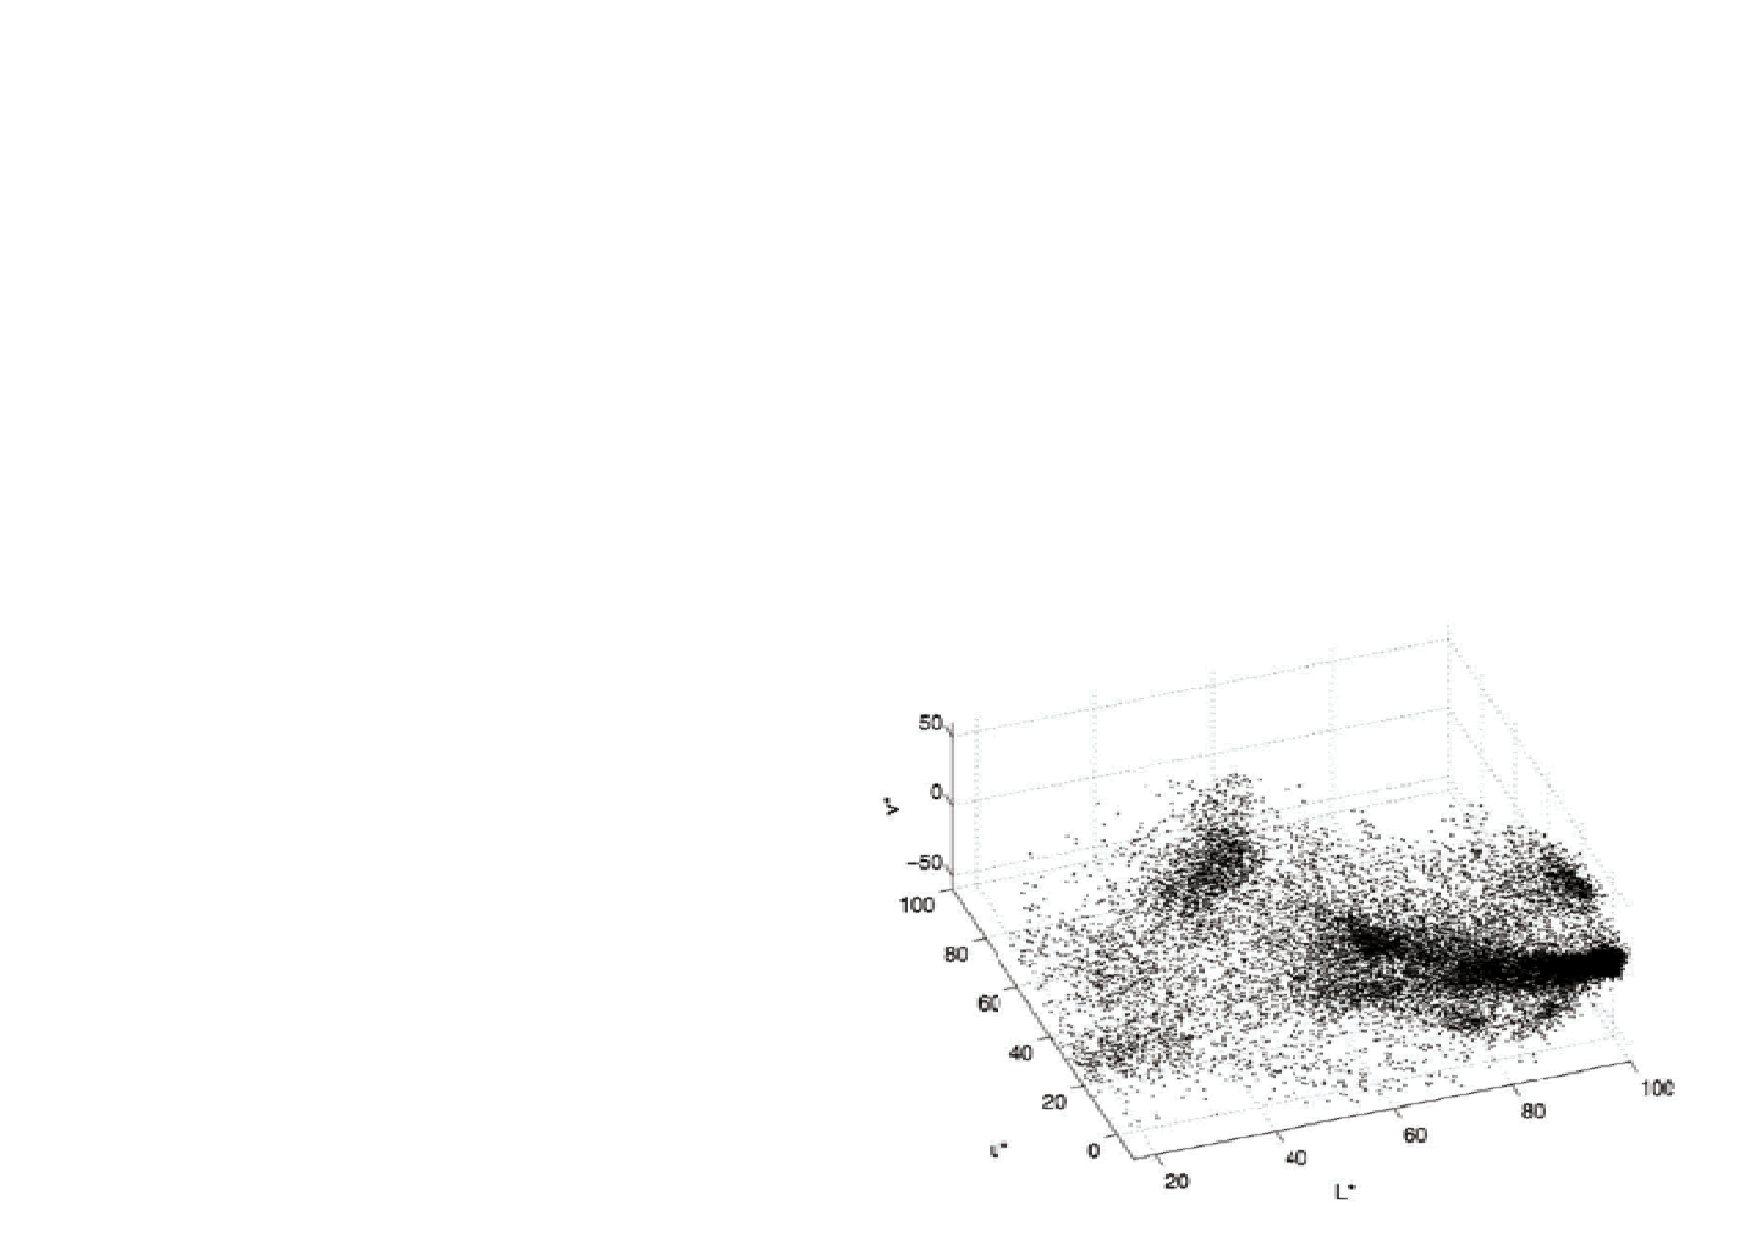
\includegraphics[width=1.0\linewidth]{images/unsupervised/non_parametric/np_2.pdf}
				%\caption{ENEL QQ-Plot Normale}
				%\label{Enel_QQ_Plot_Normal}
			\end{figure}

		\end{columns}

	%\end{block}

\end{frame}


\begin{frame}

	\frametitle{{\color{GradientDescentDiagramRed}Density-based Clustering}}

	%\begin{block}{}
		\begin{itemize}
			\item tutte le soluzioni proposte finora suggeriscono che i centri dei cluster dovrebbero essere localizzati in corrispondenza di regioni dense nello spazio delle caratteristiche
			\item al contrario, le regioni con valori di bassa densità dovrebbero essere considerate come regioni marginali
			\item i \textbf{gaussian mixture models (GMM)} rappresentano una soluzione per stimare i valori della densità attraverso un approccio  \textbf{parametrico, basato su un modello}
			\item tuttavia, il modello gaussiano non è adeguato per rappresentare i valori di densità per distribuzioni di dati generici
		\end{itemize}
	%\end{block}

\end{frame}


\begin{frame}

	\frametitle{{\color{GradientDescentDiagramRed}Density-based Clustering}}

	%\begin{block}{}

		\begin{columns}

			\column{0.67\linewidth}
			\begin{itemize}
				\item un miglioramento rispetto al clustering parametrico basato su modelli è rappresentato da \textbf{approcci di clustering non parametrici}
				\item questi operano una stima della densità nello spazio delle features senza assumere alcun modello di distribuzione specifico
					\begin{itemize}
						\item[--] una volta stimata la densità, vengono rilevati i massimi locali della funzione di densità (i massimi locali sono le \textbf{mode della distribuzione})
						\item[--] ciascuna moda è associata a una regione di influenza nello spazio delle features.\\
							La forma e l'estensione di questa regione è definita dalla forma locale della funzione di densità, non da modelli predefiniti (es. Gaussiani)
					\end{itemize}
			\end{itemize}
			\column{0.33\linewidth}
			\begin{figure}[!htbp]
				\centering
				\includegraphics[width=1\linewidth]{images/unsupervised/non_parametric/density.pdf}
				\newlinedouble
				\includegraphics[width=1\linewidth]{images/unsupervised/non_parametric/density_level_curve.pdf}
				%\caption{ENEL QQ-Plot Normale}
				%\label{Enel_QQ_Plot_Normal}
			\end{figure}

		\end{columns}

	%\end{block}

\end{frame}


\begin{frame}

	\frametitle{{\color{GradientDescentDiagramRed}Density-based Clustering}}

	%\begin{block}{}
		\begin{itemize}
%			\item in particolare, la regione di influenza di una  generica moda $q$:\\
%				comprende tutti i punti $p$ sulla superficie della funzione di densità tali che seguendo il percorso che parte da $p$ si fermano in $q$ avendo utilizzato come guida la direzione indicata del gradiente
			\item in particolare, la regione di influenza di una generica moda $q$ comprende tutti i punti $p$ sulla superficie della funzione densità tali che il percorso che parte da $p$ e segue il gradiente della superficie si ferma in $q$
		\end{itemize}

		\begin{columns}

			\column{0.5\linewidth}
			\begin{figure}[!htbp]
				\centering
				\includegraphics[width=0.85\linewidth]{images/unsupervised/non_parametric/density_red.pdf}
				%\caption{ENEL QQ-Plot Normale}
				%\label{Enel_QQ_Plot_Normal}
			\end{figure}

			\column{0.5\linewidth}
			\begin{figure}[!htbp]
				\centering
				\includegraphics[width=1.0\linewidth]{images/unsupervised/non_parametric/density_level_curve.pdf}
				%\caption{ENEL QQ-Plot Normale}
				%\label{Enel_QQ_Plot_Normal}
			\end{figure}

		\end{columns}

	%\end{block}

\end{frame}


\begin{frame}

	\frametitle{{\color{GradientDescentDiagramRed}Density-based Clustering}}

	%\begin{block}{}

		\begin{itemize}
			\item la segmentazione dell'immagine si ottiene:
				\begin{itemize}
					\item[--] associando ogni punto nello spazio delle features con la moda della regione di influenza a cui appartiene il punto
					\item[--] proiettando le regioni di influenza sull'immagine originale
				\end{itemize}
		\end{itemize}

		\begin{figure}[!htbp]
			\centering
			\includegraphics[width=1.0\linewidth]{images/unsupervised/non_parametric/meanshift_segmentation_how_works.png}
			%\caption{ENEL QQ-Plot Normale}
			%\label{Enel_QQ_Plot_Normal}
		\end{figure}

	%\end{block}

\end{frame}


\begin{frame}

	\frametitle{{\color{GradientDescentDiagramRed}Density-based Clustering}: il Mean shift}

	%\begin{block}{}

		\begin{itemize}
			\item il \textbf{mean shift} è un modello per rilevare le mode e le loro regioni di influenza nello spazio delle features
			\item sia $K_x$ la finestra di un \textbf{kernel sferico} centrata nella posizione $x$ nello spazio delle features
			\item sia $K_x(p)$ il valore del kernel $K_x$, calcolato per il punto $p$ nello spazio delle features
			\item data una distribuzione di punti nello spazio delle features $\{p_i\}$ con $i=1,...,N$; il valore medio della posizione dei punti ponderati dal kernel $K_x$, centrato in $x$ è:
				$$m(x)=\frac{\sum_i p_i K_x(p_i)}{\sum_i K_x(p_i)}$$
		\end{itemize}

	%\end{block}

\end{frame}



\begin{frame}

	\frametitle{{\color{GradientDescentDiagramRed}Density-based Clustering}: il Mean shift}

	%\begin{block}{}

		\begin{columns}

			\column{0.7\linewidth}
			\begin{itemize}
				\item si può dimostrare che il vettore di spostamento medio, definito come $m(x)-x$ è proporzionale al gradiente della stima della densità nello spazio delle features
				\item in altre parole, le iterazioni della forma $x \leftarrow m(x)$ conducono verso le mode della densità
				\item si noti che le iterazioni si fermerebbero in regioni a densità uniforme (nel caso di kernel sferico)
			\end{itemize}
			\column{0.3\linewidth}
			\begin{figure}[!htbp]
				\centering
				\includegraphics[width=1.0\linewidth]{images/unsupervised/non_parametric/mean_shift_idea.pdf}
				%\caption{ENEL QQ-Plot Normale}
				%\label{Enel_QQ_Plot_Normal}
			\end{figure}


		\end{columns}

	%\end{block}

\end{frame}


\begin{frame}

	\frametitle{{\color{GradientDescentDiagramRed}Density-based Clustering}: il Mean shift}

	%\begin{block}{}

		\begin{figure}[!htbp]
			\centering
			\includegraphics[width=0.95\linewidth]{images/unsupervised/non_parametric/mean_shift_how_works.pdf}
					%\caption{Stripe Radar for Fraud Detection}
		\end{figure}

	%\end{block}

\end{frame}


\begin{frame}

	\frametitle{{\color{GradientDescentDiagramRed}Density-based Clustering}: il Mean shift}

	%\begin{block}{}

		\begin{itemize}
			\item un'immagine è considerata come un reticolo bidimensionale di vettori d-dimensionali
				\begin{itemize}
					\item[--] d = 1 per immagini in scala di grigi
					\item[--] d = 3 per immagini a colori
					\item[--] d = 6 per la Tamura texture encoding
				\end{itemize}
			\item lo spazio del reticolo è chiamato \textbf{spatial domain} mentre lo spazio d-dimensionale è chiamato \textbf{range domain}
			\item per entrambi i domini si assume di utilizzare la metrica euclidea
		\end{itemize}


	%\end{block}

\end{frame}


\begin{frame}

	\frametitle{{\color{GradientDescentDiagramRed}Density-based Clustering}: il Mean shift}

	%\begin{block}{}

		\begin{itemize}
			\item i vettori dello \textbf{spatial e range domain} sono concatenati in uno \textbf{spatial-range domain} di dimensione $q = 2 + d$
			\item il kernel multivariato è definito come il prodotto di due kernel radiali simmetrici		\begin{itemize}
					\item[--] in questo modo il parametro della larghezza di banda può essere controllato separatamente per ciascun dominio
				\end{itemize}
		\end{itemize}

		$$K_x(p) = \frac{C}{h_s^2 h_r^d} \text{ } k\left( {\left\Vert \frac{x_s - p_s}{h_s} \right\Vert}^2 \right) k\left( {\left\Vert \frac{x_r - p_r}{h_r} \right\Vert}^2 \right)$$
	%\end{block}

\end{frame}


\begin{frame}

	\frametitle{{\color{GradientDescentDiagramRed}Density-based Clustering}: il Mean shift}

	%\begin{block}{}

		\begin{itemize}
			\item Procedura di segmentazione:
				\begin{enumerate}
					\item per ogni punto $(x_i^s, x_i^f)$ nello \textbf{spatial-range domain}, applicare la procedura del mean shift fino a convergere alla moda corrispondente $(y_i^s, y_i^f)$
					\item nell'immagine segmentata sostituire le features dell'$i$-esimo pixel con $y_i^f$.
					\item ripetere dal passaggio 1 fino a quando tutti i punti nello spazio delle features dello \textbf{spatial-range domain} sono stati elaborati
				\end{enumerate}
		\end{itemize}

		\begin{columns}

			\column{0.5\linewidth}
			\begin{figure}[!htbp]
				\centering
				\includegraphics[width=0.8\linewidth]{images/unsupervised/non_parametric/mean_shift_result_1.pdf}
				%\caption{ENEL QQ-Plot Normale}
				%\label{Enel_QQ_Plot_Normal}
			\end{figure}

			\column{0.5\linewidth}
			\begin{figure}[!htbp]
				\centering
				\includegraphics[width=0.8\linewidth]{images/unsupervised/non_parametric/mean_shift_result_2.pdf}
				%\caption{ENEL QQ-Plot Normale}
				%\label{Enel_QQ_Plot_Normal}
			\end{figure}

		\end{columns}
	%\end{block}

\end{frame}


\begin{frame}

	\frametitle{{\color{GradientDescentDiagramRed}Density-based Clustering}: segmentazione con il Mean shift}

%	\begin{block}{}
		\begin{figure}[!htbp]
				\centering
				\includegraphics[angle=0,width=0.95\linewidth]{images/unsupervised/non_parametric/meanshift_lion.pdf}
%				\caption{Single-Link Dendogram Good K}
				%\label{Enel_QQ_Plot_Normal}
			\end{figure}
%	\end{block}

\end{frame}


\begin{frame}

	\frametitle{{\color{GradientDescentDiagramRed}Density-based Clustering}: segmentazione con il Mean shift}

%	\begin{block}{}
		\begin{figure}[!htbp]
				\centering
				\includegraphics[angle=0,width=0.85\linewidth]{images/unsupervised/non_parametric/meanshift_pots.pdf}
%				\caption{Single-Link Dendogram Good K}
				%\label{Enel_QQ_Plot_Normal}
			\end{figure}
%	\end{block}

\end{frame}


\begin{frame}

	\frametitle{{\color{GradientDescentDiagramRed}Density-based Clustering}: MS, confronto con altre tecniche}

%	\begin{block}{}
		\begin{figure}[!htbp]
				\centering
				\includegraphics[angle=0,width=0.80\linewidth]{images/unsupervised/non_parametric/meanshift_compared.pdf}
%				\caption{Single-Link Dendogram Good K}
				%\label{Enel_QQ_Plot_Normal}
			\end{figure}
%	\end{block}

\end{frame}


\begin{frame}

	\frametitle{{\color{GradientDescentDiagramRed}Density-based Clustering}: MS, vantaggi e limiti}

	%\begin{block}{}

		\begin{columns}

			\column{0.6\linewidth}
			\begin{itemize}
				\item seguendo la procedura del mean shift, le regioni di influenza nello spazio delle features possono essere arbitrariamente modellate e non vengono proiettate su alcun modello particolare
				\item va però notato che il numero di cluster non è definibile a priori, bensì dipende implicitamente dalla scelta della larghezza di banda
			\end{itemize}
			\column{0.4\linewidth}
			\begin{figure}[!htbp]
				\centering
				\includegraphics[width=1.0\linewidth]{images/unsupervised/non_parametric/meanshift_number_of_clusters.pdf}
				%\caption{ENEL QQ-Plot Normale}
				%\label{Enel_QQ_Plot_Normal}
			\end{figure}


		\end{columns}

	%\end{block}

\end{frame}
